\documentclass[12pt,english]{article}
\usepackage[a4paper,bindingoffset=0.2in,%
            left=1in,right=1in,top=1in,bottom=1in,%
            footskip=.25in]{geometry}
\usepackage{blindtext}
\usepackage{titling}
\usepackage{amssymb}
\usepackage{amsmath}
\usepackage{listings}
\usepackage{lettrine} 
\usepackage{tikz}  
\usepackage{color} 
\usepackage{verbatim}
 \usetikzlibrary{shapes, arrows, calc, arrows.meta, fit, positioning} % these are the parameters passed to the library to create the node graphs  
\tikzset{  
    -Latex,auto,node distance =0.6 cm and 1.3 cm, thick,% node distance is the distance between one node to other, where 1.5cm is the length of the edge between the nodes  
    state/.style ={ellipse, draw, minimum width = 0.9 cm}, % the minimum width is the width of the ellipse, which is the size of the shape of vertex in the node graph  
    point/.style = {circle, draw, inner sep=0.18cm, fill, node contents={}},  
    bidirected/.style={Latex-Latex,dashed}, % it is the edge having two directions  
    el/.style = {inner sep=2.5pt, align=right, sloped},
         tree node/.style = {align=center, inner sep=0pt, font = \footnotesize},
every label/.append style = {font=\footnotesize},
                 PL/.style = {draw, circle, minimum size = 10mm, inner sep=0pt,
                             top color=white, bottom color=blue!20,align=center},
               ENL/.style = {% edge node left
                             font=\footnotesize, left=1pt},
               ENR/.style = {% edge node right
                             font=\footnotesize, right=1pt},
                     grow = down
}
\setlength{\parskip}{12pt}
\title{Home Work 1 Undergraduate}
\date{\today}
\author{Jose Carlos Munoz}
%================================
\begin{document}
\newgeometry{left=0.8in,right=0.8in,top=1in,bottom=1in}
\begin{center}
    \Large
    \textbf{Homework 2}\\
    \small
    \today\\
    \large
    Jose Carlos Munoz
\end{center}%===============================
3.2c)\\
\begin{equation}\tag{1}\label{eq:1}
\begin{split}
Gini_{Male} &= 1- (\frac{4}{10})^{2} - (\frac{6}{10})^{2}\\
&=0.48
\end{split}
\end{equation}
%===============================
\begin{equation}\tag{2}\label{eq:2}
\begin{split}
Gini_{Female} &= 1- (\frac{4}{10})^{2} - (\frac{6}{10})^{2}\\
&=0.48
\end{split}
\end{equation}
%===============================
\begin{equation}\tag{3}\label{eq:3}
\begin{split}
Gini_{Gender} &= \frac{10}{20}*Gini_{Male} + \frac{10}{20}*Gini_{Female}\\
&=0.48
\end{split}
\end{equation}
%===============================
The Gini for Male is as showin in\eqref{eq:1}\\
The Gini for Female is as showin in\eqref{eq:2}\\
The Gini for gender is as showin in\eqref{eq:3}\\ \\
%===============================
%===============================
3.2d)\\
\begin{equation}\tag{1}\label{eq:4}
\begin{split}
Gini_{Family} &= 1- (\frac{1}{4})^{2} - (\frac{3}{4})^{2}\\
&=0.375
\end{split}
\end{equation}
%===============================
\begin{equation}\tag{2}\label{eq:5}
\begin{split}
Gini_{Sports} &= 1- (\frac{8}{8})^{2} - (\frac{0}{8})^{2}\\
&=0.00
\end{split}
\end{equation}
%===============================
\begin{equation}\tag{3}\label{eq:6}
\begin{split}
Gini_{Luxury} &= 1- (\frac{1}{8})^{2} - (\frac{7}{8})^{2}\\
&=0.21875
\end{split}
\end{equation}
%===============================
\begin{equation}\tag{4}\label{eq:7}
\begin{split}
Gini_{Cars} &= \frac{4}{20}*Gini_{Family} + \frac{8}{20}*Gini_{Sports}+ \frac{8}{20}*Gini_{Luxury}\\
&=0.1625
\end{split}
\end{equation}
The Gini for Family is as showin in\eqref{eq:5}\\
The Gini for Sports is as showin in\eqref{eq:6}\\
The Gini for Luxury is as showin in\eqref{eq:7}\\
The Gini for Cars is as showin in\eqref{eq:8}\\ \\
%===============================
%===============================
3.2e)\\
\begin{equation}\tag{1}\label{eq:9}
\begin{split}
Gini_{Small} &= 1- (\frac{2}{5})^{2} - (\frac{3}{5})^{2}\\
&=.48
\end{split}
\end{equation}
%===============================
\begin{equation}\tag{2}\label{eq:10}
\begin{split}
Gini_{Medium} &= 1- (\frac{3}{7})^{2} - (\frac{4}{7})^{2}\\
&=\frac{24}{49}
\end{split}
\end{equation}
%===============================
\begin{equation}\tag{3}\label{eq:11}
\begin{split}
Gini_{Large} &= 1- (\frac{3}{4})^{2} - (\frac{1}{4})^{2}\\
&=0.5
\end{split}
\end{equation}
%===============================
\begin{equation}\tag{4}\label{eq:12}
\begin{split}
Gini_{Extra_Large} &= 1- (\frac{2}{4})^{2} - (\frac{2}{4})^{2}\\
&=0.5
\end{split}
\end{equation}
%===============================
\begin{equation}\tag{5}\label{eq:13}
\begin{split}
Gini_{Shirt_Size} &= \frac{5}{20}*Gini_{Small} + \frac{7}{20}*Gini_{Medium} + \frac{4}{20}*Gini_{Large} + \frac{4}{20}*Gini_{Extra_Large}\\
&=0.4914
\end{split}
\end{equation}
The Gini for Small is as showin in\eqref{eq:9}\\
The Gini for Medium is as showin in\eqref{eq:10}\\
The Gini for Large is as showin in\eqref{eq:11}\\
The Gini for Extra Large is as showin in\eqref{eq:12}\\
The Gini for Shirt Size is as showin in\eqref{eq:13}\\ \\
%===============================
%===============================
3.2f)\\
The Car type because it has the lowest Gini Index.\\\\
%===============================
%===============================
3.5a)\\
\begin{equation}\tag{1}\label{eq:14}
\begin{split}
E_{orig} &= - \frac{4}{10} *log(\frac{4}{10}) - \frac{6}{10} *log(\frac{6}{10})\\
&=.9710
\end{split}
\end{equation}
%===============================
The  overall Entropy before the split is shown in \eqref{eq:14}\\
\begin{equation}\tag{2}\label{eq:15}
\begin{split}
E_{T} &= - \frac{4}{7} *log(\frac{4}{7}) - \frac{3}{7} *log(\frac{4}{7})\\
E_{F} &= - \frac{3}{3} *log(\frac{3}{3}) - \frac{0}{3} *log(\frac{0}{0})\\
\Delta E &=E{orig} - \frac{7}{10} * E_{T} - \frac{3}{10} * E_{F}\\
 &=0.2813
\end{split}
\end{equation}
%===============================
The data gain from the splitting for A is show in \eqref{eq:15}\\
\begin{equation}\tag{3}\label{eq:16}
\begin{split}
E_{T} &= - \frac{3}{4} *log(\frac{3}{4}) - \frac{1}{4} *log(\frac{1}{4})\\
E_{F} &= - \frac{1}{6} *log(\frac{1}{6}) - \frac{5}{6} *log(\frac{5}{6})\\
\Delta E &=E{orig} - \frac{4}{10} * E_{T} - \frac{6}{10} * E_{F}\\
 &=0.2565
\end{split}
\end{equation}
%===============================
The data gain from the splitting for B is show in \eqref{eq:16}\\ \\
3.7a)\\
To find best greedy split we find which of the options gives us the least errors
\begin{equation*}\tag{1}\label{eq:17}
\begin{bmatrix} X & C1 & C2 \\0 & 60 &  60 \\1 & 40 &  40 \\ \end{bmatrix}
\end{equation*}
As seen from \eqref{eq:17},when X is 0, we see that there is a min of 60 errors and when X is 1, there is a min of 40 errors. So for X, it has an error rate of $frac{60+40}{200}$;.5\\
\begin{equation*}\tag{2}\label{eq:18}
\begin{bmatrix} Y & C1 & C2 \\0 & 40 &  60 \\1 & 60 &  40 \\ \end{bmatrix}
\end{equation*}
As seen from \eqref{eq:18}, when Y is 0, we see that there is a min of 40 errors and when X is 1, there is a min of 40 errors. So for X, it has an error rate of $frac{40+40}{200}$;.4\\
\begin{equation*}\tag{3}\label{eq:19}
\begin{bmatrix} Z & C1 & C2 \\0 & 30 &  70 \\1 & 70 &  30 \\ \end{bmatrix}
\end{equation*}
As seen from \eqref{eq:19}, when Z is 0, we see that there is a min of 30 errors and when X is 1, there is a min of 30 errors. So for X, it has an error rate of $frac{30+30}{200}$;.3\\
We split first at Z because it has the lowest error rate\par
Z=0\\
\begin{equation*}\tag{1}\label{eq:20}
\begin{bmatrix} X & C1 & C2 \\0 & 15 &  45 \\1 & 15 &  25 \\ \end{bmatrix}
\end{equation*}
As seen from \eqref{eq:20},when X is 0, we see that there is a min of 15 errors and when X is 1, there is a min of 15 errors. So for X, it has an error rate of $frac{15+15}{100}$;.3\\
\begin{equation*}\tag{2}\label{eq:21}
\begin{bmatrix} Y & C1 & C2 \\0 & 15 &  45 \\1 & 15 &  25 \\ \end{bmatrix}
\end{equation*}
As seen from \eqref{eq:20},when Y is 0, we see that there is a min of 15 errors and when X is 1, there is a min of 15 errors. So for X, it has an error rate of $frac{15+15}{100}$;.3\\
Since both are about the same, the node split can be choosen arbirtarly\par
Z=1\\
\begin{equation*}\tag{1}\label{eq:22}
\begin{bmatrix} X & C1 & C2 \\0 & 25 &  15 \\1 & 25 &  15 \\ \end{bmatrix}
\end{equation*}
As seen from \eqref{eq:22},when X is 0, we see that there is a min of 15 errors and when X is 1, there is a min of 15 errors. So for X, it has an error rate of $frac{15+15}{100}$;.3\\
\begin{equation*}\tag{2}\label{eq:23}
\begin{bmatrix} Y & C1 & C2 \\0 & 45 &  15 \\1 & 45 &  15 \\ \end{bmatrix}
\end{equation*}
As seen from \eqref{eq:23},when Y is 0, we see that there is a min of 15 errors and when X is 1, there is a min of 15 errors. So for X, it has an error rate of $frac{15+15}{100}$;.3\\
Since both are about the same, the node split can be choosen arbirtarly\par
The 2 level decision tree looks like this\\
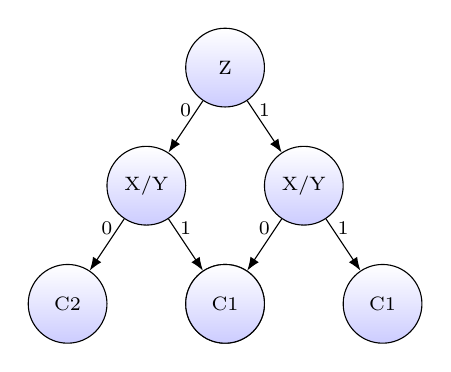
\begin{tikzpicture}
  [
    every node/.style={font=\scriptsize},
level/.style={sibling distance={4cm/max(2,#1)}}
  ]
  \node [PL] {Z}
    child{
		node [PL] {X/Y}
		child{
			node [PL] {C2}
		           edge from parent node [above, align=center]{0}}
		child{	node [PL] {C2}
 		           edge from parent node [above, align=center]{1}}
		edge from parent node [above] {0}
	}
    child{
		node [PL] {X/Y}
		child{
			node [PL] {C1}
		           edge from parent node [above, align=center]{0}}
		child{	node [PL] {C1}
 		           edge from parent node [above, align=center]{1}}
        edge from parent node [above] {1}
};
\end{tikzpicture}
\\
This Decision tree has an error of $frac{15+15+15+15}{200}$, 0.3\\
%===============================
%===============================
3.7b)\\
If we start with X instead of Z then this is how it would played out\\
X=0\\
\begin{equation*}\tag{1}\label{eq:24}
\begin{bmatrix} Y & C1 & C2 \\0 & 5 &  55 \\1 & 55 &  55 \\ \end{bmatrix}
\end{equation*}
As seen from \eqref{eq:24},when Y is 0, we see that there is a min of 5 errors and when Y is 1, there is a min of 5 errors. So for Y, it has an error rate of $frac{5+5}{100}$;.1\\
\begin{equation*}\tag{2}\label{eq:25}
\begin{bmatrix} Z & C1 & C2 \\0 & 15 &  45 \\1 & 45 &  15 \\ \end{bmatrix}
\end{equation*}
As seen from \eqref{eq:25},when Z is 0, we see that there is a min of 15 errors and when Z is 1, there is a min of 15 errors. So for X, it has an error rate of $frac{15+15}{100}$;.3\\
Since Y is has the lowest error rate, we split at Y\par
X=1\\
\begin{equation*}\tag{1}\label{eq:26}
\begin{bmatrix} Y & C1 & C2 \\0 & 35 &  5 \\1 & 5 &  35 \\ \end{bmatrix}
\end{equation*}
As seen from \eqref{eq:26},when Y is 0, we see that there is a min of 5 errors and when Y is 1, there is a min of 5 errors. So for X, it has an error rate of $frac{5+5}{100}$;.1\\
\begin{equation*}\tag{2}\label{eq:27}
\begin{bmatrix} Z & C1 & C2 \\0 & 15 &  25 \\1 & 25 &  15 \\ \end{bmatrix}
\end{equation*}
As seen from \eqref{eq:27},when Z is 0, we see that there is a min of 15 errors and when Z is 1, there is a min of 15 errors. So for X, it has an error rate of $frac{15+15}{100}$;.3\\
Since Y has the lowest rate of error, we split at Y\\
The 2 level decision tree will now looks like this\\
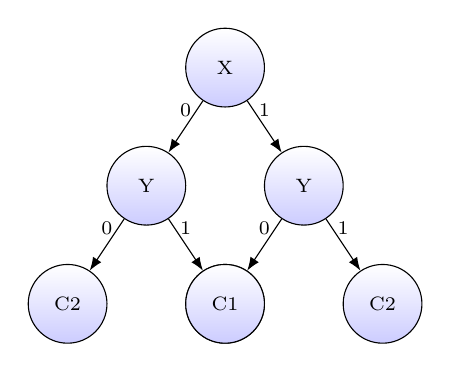
\begin{tikzpicture}
  [
    every node/.style={font=\scriptsize},
level/.style={sibling distance={4cm/max(2,#1)}}
  ]
  \node [PL] {X}
    child{
		node [PL] {Y}
		child{
			node [PL] {C2}
		           edge from parent node [above]{0}}
		child{	node [PL] {C1}
 		           edge from parent node [above]{1}}
		edge from parent node [above] {0}
	}
    child{
		node [PL] {Y}
		child{
			node [PL] {C1}
		           edge from parent node [above]{0}}
		child{	node [PL] {C2}
 		           edge from parent node [above]{1}}
        edge from parent node [above] {1}
};
\end{tikzpicture}
\\
This Decision tree has an error of $frac{5+5+5+5}{200}$, 0.1\\
3.7c)\\
We see that the decision tree for answer 3.7b has a lower error rate. This demonstrates that a greedy split is not always hueristic\\
3.8a)\\
answer 1\\
3.8b)\\
answer 1
3.8c)\\
\end{document}
